% Created 2022-04-25 Mon 14:39
% Intended LaTeX compiler: pdflatex
\documentclass[titlepage,12pt]{unisubmission}
	     \usepackage{booktabs}
	     \ClassCode{GEOL 6024}
\ClassName{GroundWater Modeling}
\ActivityType{Project}
\SubmissionType{Report}
\SubmissionNumber{1}
\SubmissionName{Github Example}
\Author{Gaurav Atreya}
\Mnumber{M14001485}
\Keywords{Groundwater,Modeling,Flopy}
\author{Gaurav Atreya}
\date{\today}
\title{Github Example for Flopy}
\hypersetup{
 pdfauthor={Gaurav Atreya},
 pdftitle={Github Example for Flopy},
 pdfkeywords={},
 pdfsubject={},
 pdfcreator={Emacs 28.1 (Org mode 9.5.2)}, 
 pdflang={English}}
\begin{document}

\maketitle
\setcounter{tocdepth}{2}
\tableofcontents
\section{Introduction}
\label{sec:org97f6941}
This model is very basic model on a simple grid to show what flopy can do, and be familiar with the functions and classes in flopy. We'll use the model from the flopy github readme, and make and run the model. It's mostly to confirm your installation of modflow and flopy are correct and any code we write for other exercises will be run properly.

\section{Code}
\label{sec:orgf5c47b5}

\subsection{Importing Libraries}
\label{sec:org393517c}
First Let's load libraries, flopy is the flopy library and matplotlib is for plotting the plots, flopy also uses this internally for the plots.

\begin{minted}[]{python}
import flopy
import matplotlib.pyplot as plt
\end{minted}

\subsection{Flopy model}
\label{sec:org68176e2}
We also need to define the working directories flopy will save the modflow model in that directory with given name. Here we also give the exe\textsubscript{name} which is the modflow executable to be called for simulation.

\begin{minted}[]{python}
ws = './models/01_github_example/'
name = '01_git_ex'
sim = flopy.mf6.MFSimulation(sim_name=name, sim_ws=ws, exe_name='modflow-mf6')
\end{minted}


After we have a simulation object, we can add more packages. Here tdis package is for time descretization we're using the default values as we don't have timesteps.

I don't know what ims package does.

gwf is groundwaterflow package.
\begin{minted}[]{python}
tdis = flopy.mf6.ModflowTdis(sim)
ims = flopy.mf6.ModflowIms(sim)
gwf = flopy.mf6.ModflowGwf(sim, modelname=name, save_flows=True)
\end{minted}


Here we define descretization package which will take number of rows and columns and make a grid internally.
We're using 10x10 grids.

\begin{minted}[]{python}
dis = flopy.mf6.ModflowGwfdis(gwf, nrow=10, ncol=10)
ic = flopy.mf6.ModflowGwfic(gwf)
npf = flopy.mf6.ModflowGwfnpf(gwf, save_specific_discharge=True)
\end{minted}


Now we can use chd package which is used for constant head conditions, we have assigned two points with heads 1 and zero we we can see the flow from higher head to lower.

\begin{minted}[]{python}
chd = flopy.mf6.ModflowGwfchd(gwf, stress_period_data=[[(0, 0, 0), 1.],
                                                       [(0, 9, 9), 0.]])
\end{minted}

Now the oc package will be used to give the filenames for where the results will be saved. We can load these files directly and use the data next time if running model everytime is troublesome.

\begin{minted}[]{python}
budget_file = name + '.bud'
head_file = name + '.hds'
oc = flopy.mf6.ModflowGwfoc(gwf,
                            budget_filerecord=budget_file,
                            head_filerecord=head_file,
                            saverecord=[('HEAD', 'ALL'), ('BUDGET', 'ALL')])
\end{minted}

After we have all the packages we use \texttt{write\_simulation()} function to write the files for the simulation that will be used my modflow when we use \texttt{run\_simulation()}.

\begin{minted}[]{python}
sim.write_simulation()
sim.run_simulation()
\end{minted}

\begin{minted}[]{text}
| True | nil |
\end{minted}


The output of \texttt{run\_simulation()} is \texttt{True}, hence the model run was successful.

We can extract the values from the model. We can also extract them using the output files we saved using oc package.

\begin{minted}[]{python}
head = gwf.output.head().get_data()
bud = gwf.output.budget()
\end{minted}

The output files for head and bud are binary files and are quite hard to read (even more so because 3D data are compressed to 1D), so we're going to use postprocessing tools to get the data we want. Let's get the specific discharge values so we can use them to plot arrows in the plan to show the direction of flow.

\begin{minted}[]{python}
spdis = bud.get_data(text='DATA-SPDIS')[0]
qx, qy, qz = flopy.utils.postprocessing.get_specific_discharge(spdis, gwf)
\end{minted}

Now we can use model structure and the output to make plots.

\begin{minted}[]{python}
pmv = flopy.plot.PlotMapView(gwf)
pmv.plot_array(head)
pmv.plot_grid(colors='white')
pmv.contour_array(head, levels=[.2, .4, .6, .8], linewidths=3.)
pmv.plot_vector(qx, qy, normalize=True, color="white")
\end{minted}

If you want to save the figure use this. You can save png or pdf. You can use \texttt{plt.show()} to view it.
\begin{minted}[]{python}
plt.savefig("./images/1_results_plan.pdf")
plt.show()
\end{minted}

\begin{center}
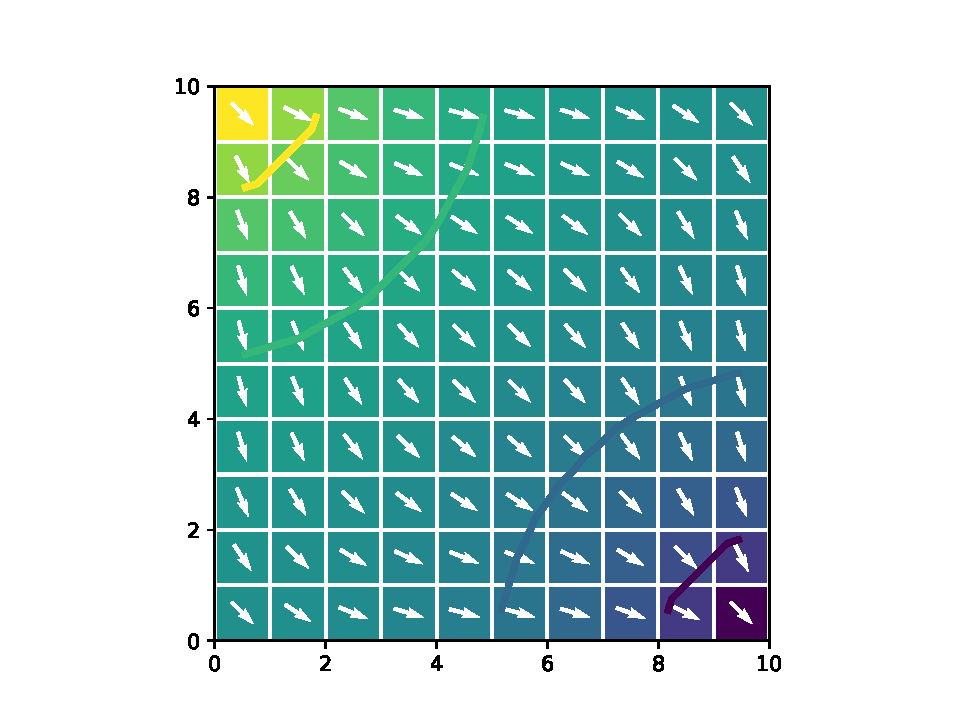
\includegraphics[width=.9\linewidth]{./images/1_results_plan.pdf}
\end{center}

We got the result which is same as that in the example. So it was a success.

\subsection{Zone budget}
\label{sec:org13d2fc5}
We hadn't imported numpy so let's do that.

\begin{minted}[]{python}
import numpy as np
\end{minted}

We'll make a array with same shape as grid and put some arbitrary cells as different zones.

\begin{minted}[]{python}
zones = np.ones((10, 10), dtype=int)
zones[(1, 1)] = 2
zones[(2, 2)] = 2
zones[(7, 7)] = 3
zones[(8, 8)] = 3
\end{minted}

Make a zonebudget model.

\begin{minted}[]{python}
bm = gwf.output.zonebudget(zones)
bm.change_model_name(name)
bm.change_model_ws(ws)
\end{minted}

Write input files and run it.

\begin{minted}[]{python}
bm.write_input()                # see NOTE
bm.run_model(exe_name='modflow-zbud6')
\end{minted}

\begin{minted}[]{text}
| True | nil |
\end{minted}

NOTE: The \texttt{bm.write\_input()} has a bug and doesn't write the grb file and it'll end up being an error. \href{https://github.com/modflowpy/flopy/issues/1395}{I brought it to the attention of the developers and they've fixed it}. But it's not yet available to the pip version 3.3.5. If the next version isn't yet released when you're trying out, then you can install the git's latest version with \texttt{pip install -{}-upgrade git+https://github.com/modflowpy/flopy.git} in your terminal.

Now we can get the zonebudget for the model.

\begin{minted}[]{python}
bm.get_budget()
\end{minted}

\begin{minted}[]{text}
| 1 | 0 | 0 | DATA_SPDIS_IN  |          0 |          0 |          0 |
| 1 | 0 | 0 | CHD_IN         | 0.33205402 |          0 |          0 |
| 1 | 0 | 0 | DATA_SPDIS_OUT |          0 |          0 |          0 |
| 1 | 0 | 0 | CHD_OUT        | 0.33204178 |          0 |          0 |
| 1 | 0 | 0 | FROM_ZONE_0    |          0 |          0 |          0 |
| 1 | 0 | 0 | FROM_ZONE_1    |          0 |   0.214903 | 0.21490513 |
| 1 | 0 | 0 | FROM_ZONE_2    | 0.21488982 |          0 |          0 |
| 1 | 0 | 0 | FROM_ZONE_3    | 0.21490489 |          0 |          0 |
| 1 | 0 | 0 | TO_ZONE_0      |          0 |          0 |          0 |
| 1 | 0 | 0 | TO_ZONE_1      |          0 | 0.21488982 | 0.21490489 |
| 1 | 0 | 0 | TO_ZONE_2      |   0.214903 |          0 |          0 |
| 1 | 0 | 0 | TO_ZONE_3      | 0.21490513 |          0 |          0 |
\end{minted}

\section{Export to vtk format}
\label{sec:org51ec253}

We can also export the heads data we obtained from the simulation and then visualize it using external tools like Paraview.

\begin{minted}[]{python}
import os
from flopy.export import vtk
vtk.export_heads(sim.get_model(), os.path.join(ws, head_file), ws, smooth=False, kstpkper=[(0,0)], point_scalars=False, nanval=-1e30)
\end{minted}

After running the code we get a \texttt{.vtk} file in the same directory as the model files, after that we can load it in Paraview, as seen in figure below.

\begin{figure}[htbp]
\centering
\includegraphics[width=.9\linewidth]{./images/paraview-sc-1.png}
\caption{Visualization of Heads in Paraview.}
\end{figure}
\end{document}